\begin{frame}[fragile]{Uso de SurfaceView en Android}
\textbf{¿Qué es SurfaceView?}

\begin{itemize}
    \item Es un componente que permite dibujar directamente sobre una superficie separada del hilo principal (UI thread).
    \item Ideal para gráficos en tiempo real como videojuegos, animaciones o streaming de video.
\end{itemize}

\textbf{Componentes clave:}
\begin{itemize}
    \item \textbf{SurfaceHolder:} Controla la superficie de dibujo.
    \item \textbf{Canvas:} Permite realizar los dibujos.
    \item \textbf{Thread:} Maneja el ciclo de renderizado.
\end{itemize}

\textbf{Métodos principales (SurfaceHolder.Callback):}
\begin{itemize}
    \item \textbf{surfaceCreated():} Se invoca cuando la superficie está lista para dibujar.
    \item \textbf{surfaceChanged():} Se ejecuta cuando cambia tamaño o formato.
    \item \textbf{surfaceDestroyed():} Se llama cuando la superficie se destruye.
\end{itemize}

\textbf{Ventajas:}
\begin{itemize}
    \item Alto rendimiento para gráficos.
    \item Control directo del renderizado.
\end{itemize}

\end{frame}




\begin{frame}[fragile]{Drag and Drop y SurfaceView en Android}
\textbf{¿Qué es Drag and Drop?}

\begin{itemize}
    \item Es una técnica de interacción que permite arrastrar (drag) y soltar (drop) elementos en la pantalla.
\end{itemize}

\textbf{Implementación en Android:}
\begin{itemize}
    \item Uso de eventos táctiles (\texttt{onTouchEvent}).
    \item Manejo de coordenadas (X, Y) para actualizar la posición del objeto.
    \item Uso de \texttt{setOnDragListener()} en vistas estándar.
\end{itemize}

\vspace{0.3cm}

\textbf{Relación con SurfaceView:}
\begin{itemize}
    \item En \textbf{SurfaceView} el control es manual:
    \begin{itemize}
        \item Se capturan eventos táctiles.
        \item Se redibuja el objeto en nuevas posiciones usando \texttt{Canvas}.
    \end{itemize}
\end{itemize}


\textbf{Ventajas:}
\begin{itemize}
    \item Ideal para juegos o interfaces dinámicas. Permite interacción intuitiva y mayor control en SurfaceView para animaciones en tiempo real.
\end{itemize}

\end{frame}




\begin{frame}[fragile]
\frametitle{Demo 17: Surface View }
\begin{columns}
\column{0.80\linewidth}

\scriptsize
Del Repositorio Github:
\begin{itemize}
%\item Agregar la siguiente linea: \textit{implementation("com.github.PhilJay:MPAndroidChart:v3.1.0")}, al final de la seccion Dependencies del archivo Build.graddle.kts (Module: App).
%\item Agregar la siguiente linea: \textit{maven \{ url = uri(``https://jitpack.io'') \}}, al final de la seccion \textit{dependencyResolutionManagement } del archivo settings.graddle.kts.
\item Copiar el archivo \textit{MainActivity\_Demo17.java} (dentro del Folder códigosJAVA) al mismo directorio donde esta el MainActivity.java
\item Copiar los archivos \textit{DragAndDropView.java, DragAndDropThread.java, Circulo.java, Figura.java y Rectangulo.java},  (dentro del Folder códigosJAVA) al mismo directorio donde esta el MainActivity.java
\item Copiar el archivo \textit{activity\_main\_demo17.xml} (dentro del Folder Carpeta\_layout) al mismo directorio donde esta el activity\_main.xml
\item Modificar dentro del archivo \textit{activity\_main\_demo17.xml} la cadena \textit{.com.example.a2026\_01\_holamundoandroid.DragAndDropView} por \textit{$<$SuPackage$>$.DragAndDropView}.
\item Modificar en el archivo \textit{AndroidManifest.xml} la cadena \textit{.MainActivity\_Demo16} por \textit{.MainActivity\_Demo17}.


%\item Ir a la linea 22 de archivo del archivo \textit{MainActivity\_Demo09.java}, poner el cursos en la palabra (en Rojo) \textit{documentfile}, presionar la combinación ALT+ENTER, y seleccionar de la lista desplegable la opcion ``Add dependency on ....''. Esto quitará el error y hara los ajustes necesarios. 
\end{itemize}

%\begin{block}{Demo \#09}
%Un App que permite escribir el contenido de un EditText a un archivo y cargar el contenido de cualquier archivo en el EditText
%\end{block}


\column{0.20\linewidth}

\begin{center}
 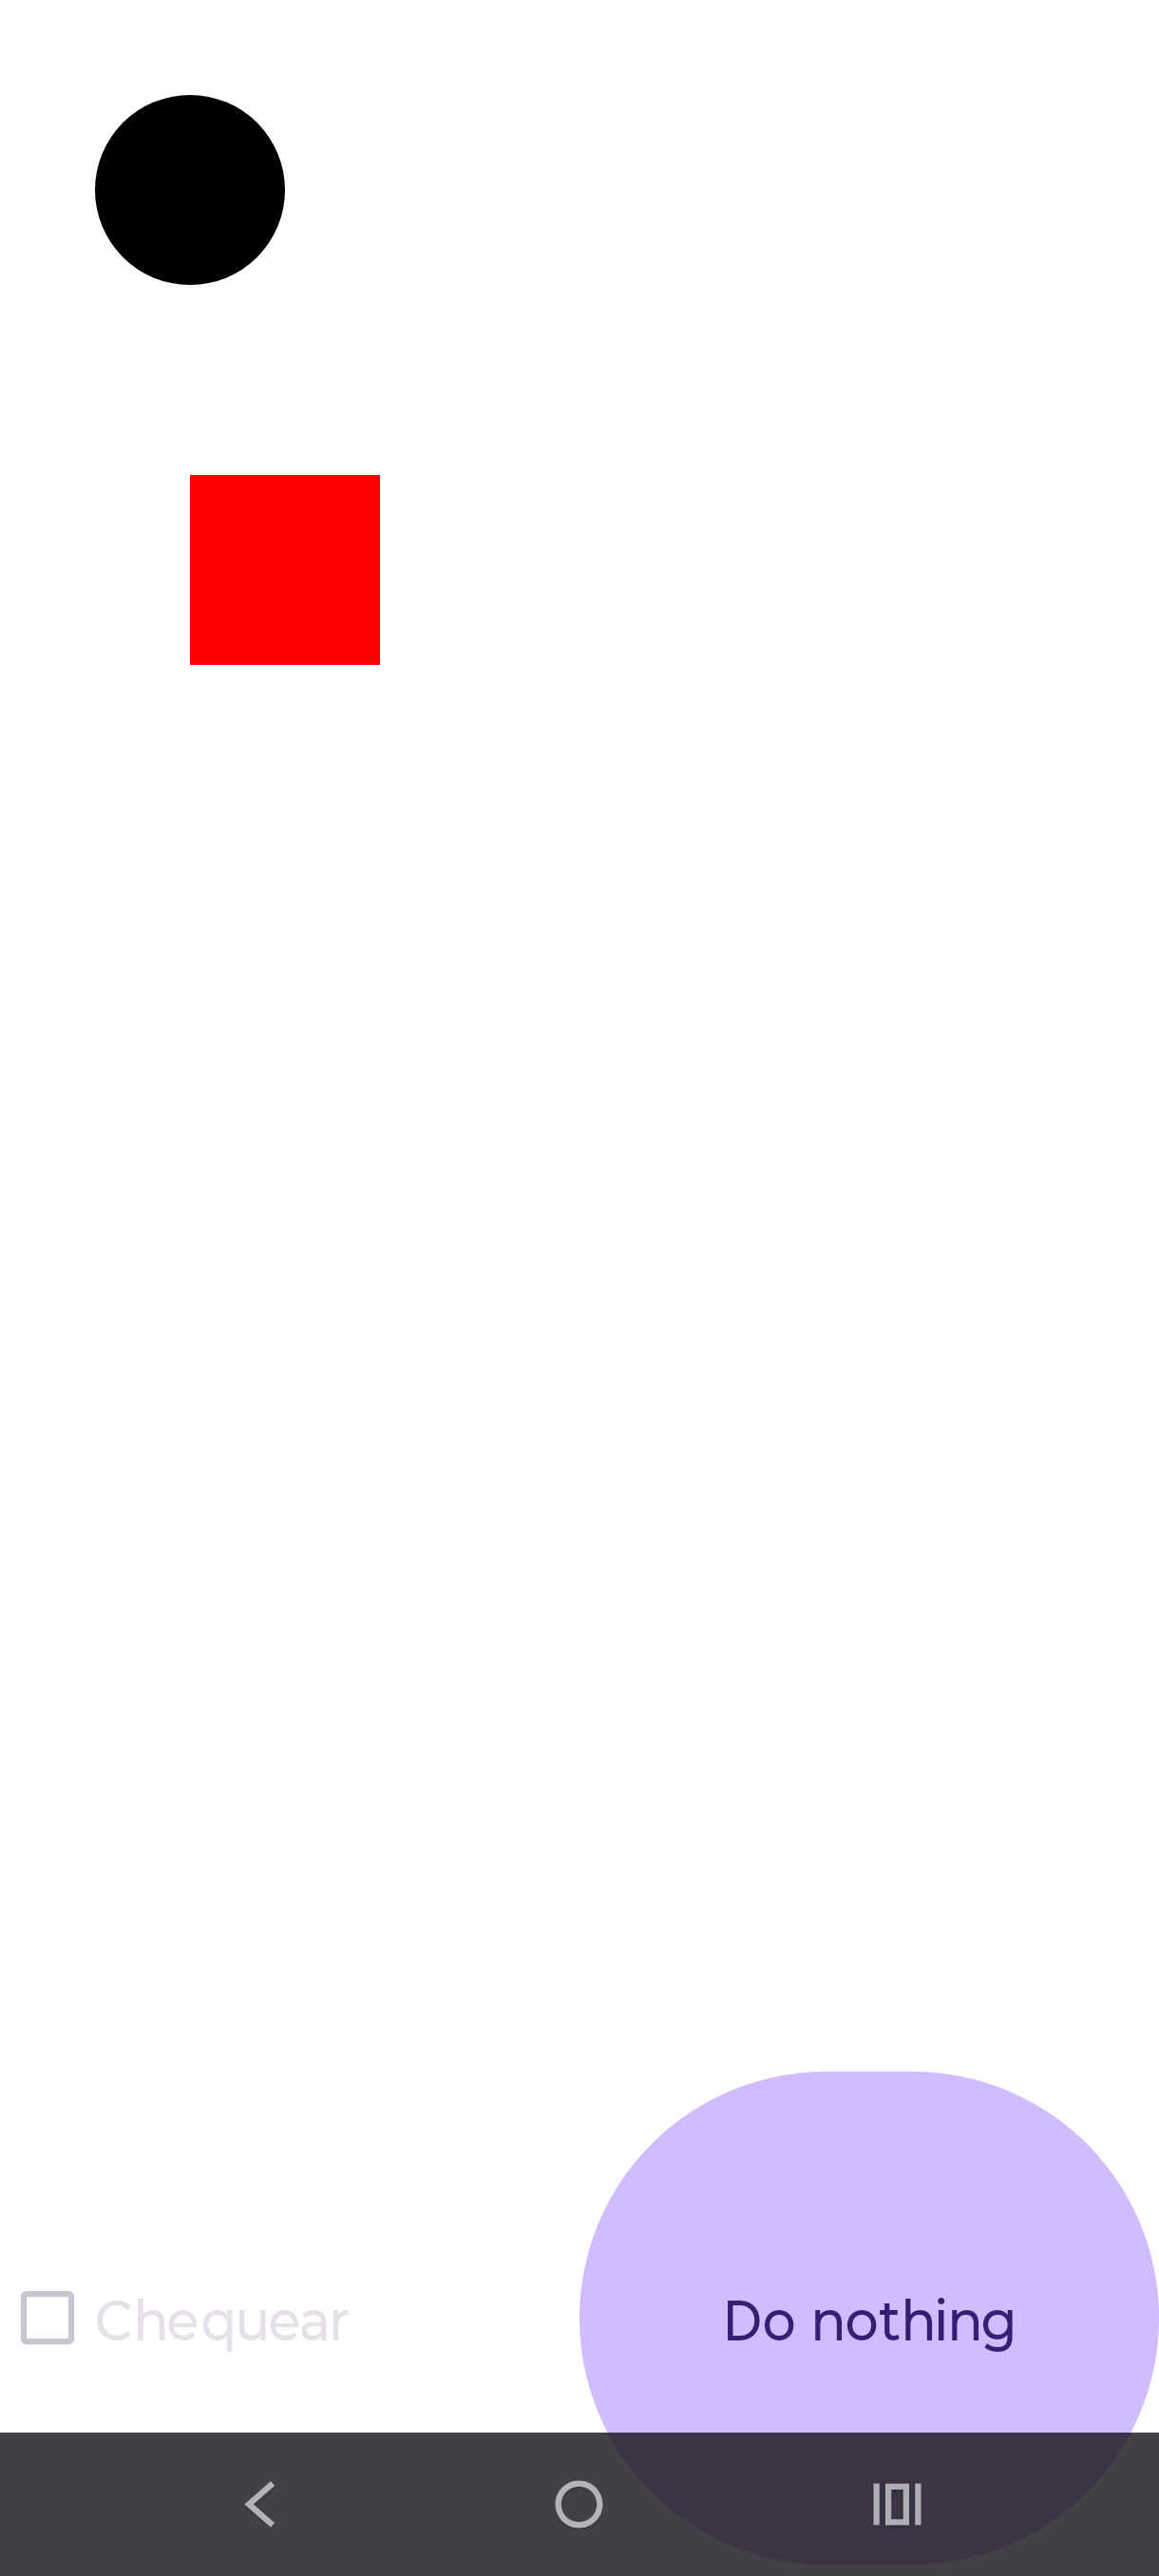
\includegraphics[width=0.98\textwidth]{02_TallerCBTis/figs/Demo17}
\end{center}

\end{columns}

\end{frame}

